
\section{Julia implementation}\label{sec:julia}

The computer code is implemented in Julia language~\cite{BEKS14} according to the workflow described below, whose stages are parallelized and/or optimized in various ways. The workflow scheme can be seen in Fig. \ref{fig:schema}. The implementation is available on GitHub \cite{larsurf-github} and our \texttt{LarSurf.jl} package can be installed using a standard Julia package register.

\subsection{Parallel workflow}\label{sec:implementation}


\paragraph{Workflow setup}\label{sec:workflow}
The functions in this preliminary step include:
\begin{enumerate}

\item input of 3D medical image $\mathcal{I}$ with \emph{shape} $(\ell_1, \ell_2, \ell_3)$, such that: $\mathcal{I} = [\ell_1]\times[\ell_2]\times[\ell_3]$, where $[\ell_k] = [1,2,\ldots,\ell_k]$;

\item analysis of resources available in the computational environment, including operating system, type and number of compute nodes (processors, cores, GPUs), number of cores per node, RAM and cache amounts;

\item depending on the above, best choice of the \emph{size} of 3D image brick $\mathcal{B}$. With default $\emph{size}=64$,  the \emph{number of bricks} will be $n=\ceil{\ell_1/size}\times\ceil{\ell_2/size}\times\ceil{\ell_3/size}$. 
Hence the default \emph{number} of bricks, of size $64^3$, is $m=8\times 8\times 4 = 256$, for standard medical images $512\times 512\times 256$;

\sloppy{
\item computation of sparse brick boundary matrix $[\partial_B]$, where \texttt{Int8} and \texttt{Int64} are the types for values and indices, returning a sparse matrix value of type \texttt{SparseMatrixCSC\{Int8\}\{Int64\}}, stored by Compressed Sparse Column (CSC) format. The storage of $[\partial_B]$ (for $\emph{n}$ = 64) requires about 12\,MB;
}

\item creation of either a local or distributed \texttt{channel} to implement a producer/consumer model of parallel/distributed computation, depending on available resources;

\item distribution of matrix $[\partial_B]$, of default size 12\,MB, to all available nodes/cores (Julia workers), using the Julia macro \texttt{@eveywhere}. 

\end{enumerate}

\begin{figure}[tbp]
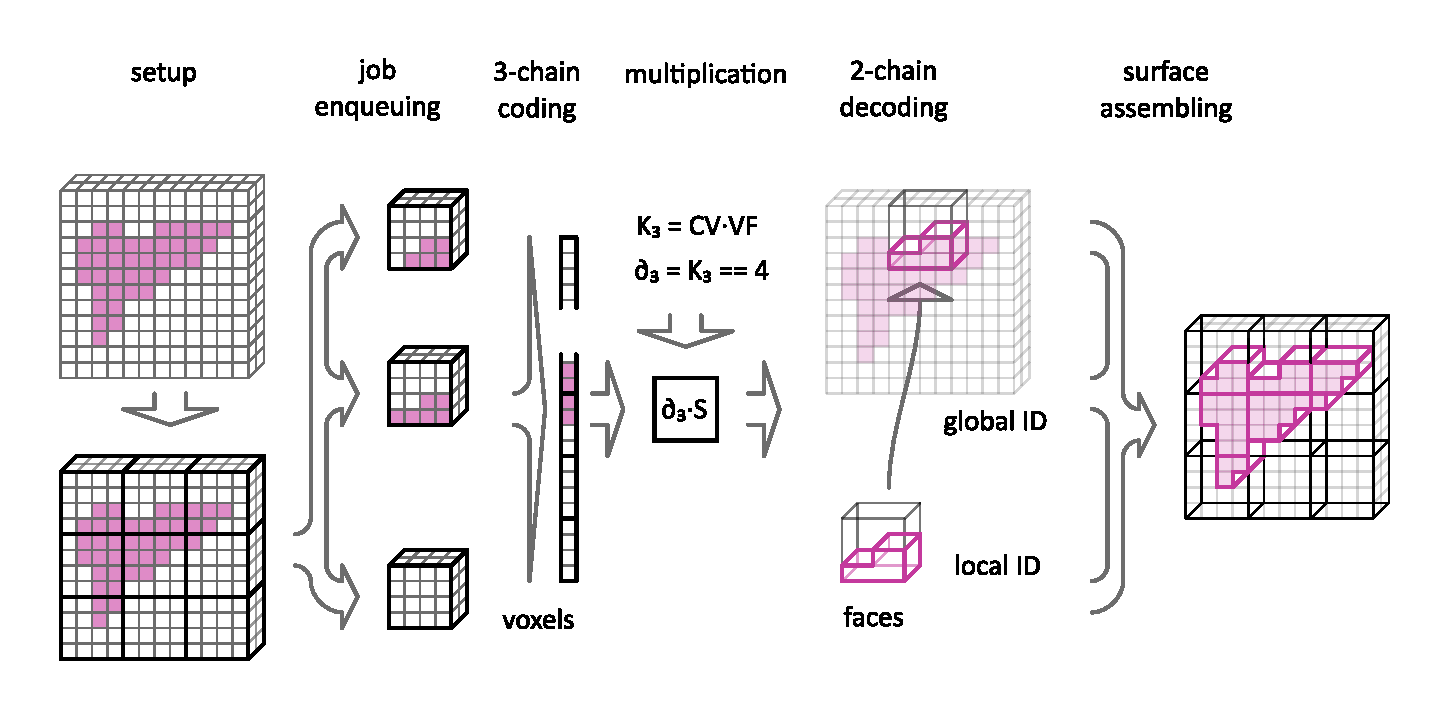
\includegraphics[width=\textwidth]{figs/schema_horizontal.pdf} 
%\includegraphics[scale=1]{input/ircad_comparison.pdf} 
\caption{Workflow of \textsc{lar-surf} algorithm}
\label{fig:schema}
\end{figure}

%With $size=64$, the number of non-zeros within the sparse matrix $[\partial(64^3)]$ is $\mathtt{nnz} = 4\,792\,266$, for a memory size of $9\times \mathtt{nnz}+8\times 262144 \simeq 45$ MB. The memory size of the sparse matrix is computed by considering $8+1$ bytes for non-zero element (which are exactly 6 per row), plus 8 bytes per each index of column start.  


\paragraph{Job enqueuing}
% \subsubsection{Job enqueuing}
\label{sec:job-enq}
Communication and data synchronization are managed through \emph{Channels}, which are the FIFO conduits that may provide producer/consumer communication. Overall execution time can be improved if other tasks can be run while a task is being executed, or while waiting for an external service/function to complete. The single work items of this stage follow:
\begin{enumerate}

\item extraction, from image arrays of the block views, depending on 3 Cartesian indices;

\item transform  each block \emph{from global} $[\ell_1]\times[\ell_2]\times[\ell_3]$ to \emph{local coordinates} $[n]\times[n]\times[n]$;

\item further transform of each \emph{foreground voxel} $\nu\in\mathcal{S}\subseteq\mathcal{I}$ from Cartesian to linear coordinates, using suitable functions from Julia's library.

\item enqueuing the job (as a sequence of integer positions for the non-zero image elements aligned in a memory buffer of proper \texttt{Channel} type).
\end{enumerate}

\paragraph{3-Chain encoding}
\label{chain-coding}
The interesting part of the \emph{Image} $\mathcal{I}$ is called \emph{Segment} $\mathcal{S}$. The goal of the whole \emph{workflow} is to extract a \emph{boundary model} of $\mathcal{S}$ from $\mathcal{I}$. The portion of $\mathcal{S}$ inside $\mathcal{B}$, will be denoted as $\mathcal{S}(B)$.
Each block $\mathcal{B}$ of the 3D image must by converted into the \emph{coordinate representation} of a vector $\nu\in C_3$ in the linear space  of 3-chains. 

In coordinates local to $\mathcal{B}$, once an ordering from Cartesian to linear coordinates has been fixed, this vector is represented by a \emph{binary array} of length $size^3$. With $size=64$, we have $64^3=262144$,  with a non-zero value (i.e.~$1$) for each foreground voxel in $\mathcal{S}(B)$. Therefore, the coded segment portion $\mathcal{S}(B)$ results in a space occupancy of about $262$ KB if encoded as a full array (i.e.,~including zero values). When encoded as a sparse vector, its space occupancy will correspondingly decrease.

\begin{enumerate}

\item each encoding task produces either a full or sparse binary vector. 
We get either 262 KB or less per job, depending on the use of either a full vector, or a sparse one;

\item a special format for sparse CSC (Compressed Sparse Column) vectors can be used, since the \emph{value} data for non-zeros does not need storage. Hence only a single 1-array of \texttt{Int64} row positions (with total length equal to the number of non-zeros in the block, with $8\times\mathtt{nnz}$ kB storage) is needed;

\item prepare sequences of such data vectors, in order to feed efficiently the available processor threads.
\item In case of presence of one/more GPUs, a smaller size of the block is preferable for speed, even with smaller boundary matrices and higher numbers of coded vector chains.

\end{enumerate}

\paragraph{SpMM Multiplication}\label{SpMM-multiplication}
According to current literature~
\cite{Buluc2017}, it is more convenient to execute SpMV (sparse matrix-vector) multiplications than SpMSpV (sparse matrix-sparse vector) multiplications. Since we have 256 such jobs (one multiplication per block) to perform in the default setting of the algorithm (
size of the block $64^3$; the size of the image $512^2\times 256$), or more in case of either smaller blocks or image larger than the standard one, this stage must be evidently parallelized and carefully tuned, possibly by using the GPU, if available.
\begin{enumerate}

\item the total speed of this stage is strongly dependent on the hardware available, on the granularity of bricks, and on the choice between dense/sparse storage of encoded 3-chains;

\item the compute elements or threads is fed without solution of continuity in a \emph{dataflow} process. This parallel operation is, according to our preliminary experiments, the critical one of the whole workflow, since any $\Delta T$ (either positive or negative) in this stage contributes to the total time $T$.

\end{enumerate}

\paragraph{2-Chain decoding}\label{sec:two-chain-decoding}
Each multiplication of $[\partial_B] : C_3 \to C_2$, times a 3-chain $\nu\in C_3$, produces a 2-chain  $\sigma\in C_2$, i.e.,~the \emph{coordinate representation} of the \emph{boundary vector} $\sigma\in C_2$.  The inverse of the coding algorithm is executed in the present stage.  This process can also be partially superimposed in time with the previous ones, depending on the size of the memory buffers used to feed the CPU cores or the GPUs and get their results. Its elementary steps are as follows:

\begin{enumerate}

\item reading of position of ones (non-zeros) in the 2-chain as linear indices of rows;

\item conversion from linear indices to Cartesian indices in coordinates local to the $\mathcal{B}$ block, using the appropriate library functions;

\item conversion from each Cartesian index value to a suitably oriented (i.e.,~with proper attitude) geometry quadrilateral (or pair of triangles) in local coordinates.

\end{enumerate}

Julia's vectorized pipeline data-flow was 
the more appropriate model to feed the workers' jobs.

\paragraph{Assembling and artifact filtering}\label{sec:artifact-filtering}
The results of the previous stages can be described as a \emph{collection of sets} of \emph{geometric quadrilaterals (quads)}, each one encoded as an array of quadruples of integer indices, pointing to the linear array of grid vertices associated with the image block $\mathcal{B}$.  In other words, \emph{all quads} of \textbf{each job} are now given in the \textbf{same} \emph{local coordinates}.  Besides putting each partial surface $\mathcal{S}(B) = (\texttt{V}_B, \texttt{FV}_\sigma)$ in the global coordinate system of the image, the present stage must eliminate the redundant boundary features possibly generated at the edges of the partial surface $\mathcal{S}(B)$ within each block $\mathcal{B}$:

\begin{enumerate}

\item translate each array $\mathtt{FV}_\sigma$, of type \texttt{Lar.Cells}, by summing each vertex index to the linearized offset of the Cartesian coordinates $(i,j,k)$ of the $\mathcal{B}$'s \emph{reference vertex}, i.e.,~the one with lowest \emph{Cartesian coordinates} within the $\mathcal{B}$ block.

\item remove both instances of \emph{double quads} generated by \texttt{Lar} software at the block boundaries 
(see Fig.~\ref{fig:brickboundary}). 
% TODO fix reference probably uncomment next line to link it to Figure 3
% (see Figure~\ref{fig:example}). 
These are artifacts generated by the decomposition of the whole image into a number of blocks of tractable size.

\item 
a smart strategy to remove such artifacts was used, that does not require any sorting nor searching on the assembled array of quads. The output set of 2-cells (or triangles) is just rewritten, discarding the elements pointing to all vertices with one coordinate equal to a block boundary. A proper software filter was applied to this purpose.
% The details of this \emph{artifact filtering} are elucidated in  section~\ref{sec:covering}.
% TODO fix the reference
% TODO is there such a section?

\end{enumerate}

\paragraph{Smoothing}\label{sec:smoothing}
The final smoothing of the generated surfaces cannot be performed block-wise since this would introduce non-smooth artifacts at the block boundaries. Anyway, Taubin smoothing~\cite{Taubin1995} can be performed in parallel, since for each vertex in the final surface (except eventually the ones on the image $\mathcal{I}$ boundaries) it essentially consists in computing a new position as a proper average of its neighboring vertices, i.e.,~by applying a discrete Laplacian operator.  Some appropriate sets of workers may so be assigned the task of generating iteratively a new position for the vertices they take cure of. In particular, we have:
\begin{enumerate}

\item job enqueuing, by writing sets of integers (global linear indices of vertices) in array buffers of type \texttt{Channel};

\item vectorized computation of proper averages of near vertices;

\item job dequeuing, by recovering finished tasks from a channel and assembling the results into the embedding function $\mathtt{V}: C_0 \to \E^3$, providing an array of type \texttt{Lar.Points} of \texttt{Float64 $\times$ 3}, with vertex coordinates by column.
\end{enumerate}



\subsection{Performance analysis}\label{sec:analysis}

\paragraph{Boundary matrix size}
The size of the boundary matrix is a critical parameter of the \textsc{lar-surf} method. To determine the optimal size of the boundary matrix we experimented on artificial data (Fig.  \ref{fig:bm_size_tesla}). The size of the experimental data was set to $512\times512\times512$ (a typical size of Computed Tomography medical images). Computation was done on the Tesla DGX-1 machine.

According to the experiment the fastest computation is with boundary matrix size $64\times64\times64$. This is an expected result. The larger boundary matrix is too big to fit in CPU's cache memory.

\begin{figure}
\centering
\begin{subfigure}{0.495\textwidth}
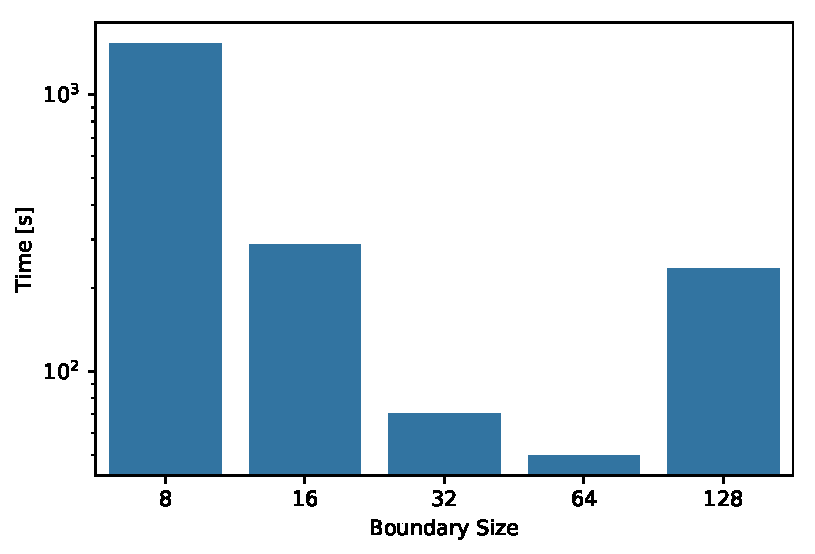
\includegraphics[width=0.99\textwidth]{figs/bm_size_tesla.pdf} 
%\includegraphics[scale=1]{input/ircad_comparison.pdf} 
\subcaption{Time requirements of the \textsc{lar-surf} filter used on artificial volumetric data with various sizes of boundary matrix}
% \caption{Time requirements of LAR-SURF filter used on artificial with different size of boundary matrix}
\label{fig:bm_size_tesla}
\end{subfigure}
\begin{subfigure}{0.495\textwidth}

\includegraphics[width=0.99\textwidth]{figs/ircad_comparison.pdf} 
%\includegraphics[scale=1]{input/ircad_comparison.pdf} 
\subcaption{Time requirements of the LAR-SURF filter and Marching Cubes on the Ircad dataset. Error bars show the 95\% confidence interval}
\label{fig:ircad_comparison}
\end{subfigure}
\caption{Performance analysis of the \textsc{lar-surf} filter.}

\end{figure}


\paragraph{Comparison with the Marching Cubes algorithm}
To compare the time requirements of \textsc{lar-surf} with Marching Cubes implemented in Python we performed an experiment on Ircadb dataset \cite{ircadb}. Dataset contain 20 Computed Tomography images (see table \ref{tab:ircad2}) with xy-resolution from 0.56 mm to 0.87 mm and z-resolution from 1.0 mm to 4.0 mm. 
The number of slices is each series varies from 74 to 260 and the size of each slice is $512\times512$. 
The dataset contains manually segmented liver, portal vein, and other structures. We performed surface extraction of the liver with Marching Cubes and LAR-SURF. The time required for computation can be seen in Fig. \ref{fig:ircad_comparison}. 

Based on the t-test with $\alpha=0.99$, $p=\num[]{8.735e-24}$ and 
$s=\num[]{-16.67}$ it can be shown that the mean time consumed by LAR-SURF is significantly smaller than that consumed by Marching Cubes.


% \begin{figure}
% \centering
% \includegraphics[width=0.99\textwidth]{figs/ircad_comparison.pdf} 
% %\includegraphics[scale=1]{input/ircad_comparison.pdf} 
% \caption{Time requirements of LAR-SURF filter and Marching Cubes on Ircad dataset. Error bars shows the 95\% confidence interval}
% \label{fig:ircad_comparison}
% \end{figure}

